% !TEX program = xelatex
\documentclass[UTF8, 10pt]{ctexrep}

% 编程
\usepackage{ifthen}

% 颜色
\usepackage[dvipsnames]{xcolor}

% 字体
\usepackage{fontspec}
% \setmainfont[BoldFont={SourceHanSansSC-Medium}]{Source Han Serif SC}
\setCJKmainfont{Source Han Serif SC}
% \setsansfont[BoldFont={SourceHanSansSC-Bold}]{Source Han Sans SC}
\setCJKsansfont{Source Han Sans SC}
% \setCJKmonofont[BoldFont={Kaiti SC Bold}]{Kaiti SC Regular}

% 中文排版设置
\ctexset{
    space=true,
    punct=quanjiao,
    chapter/number = \arabic{chapter},
    chapter/numberformat = \color{blue}\zihao{0}\itshape,
    chapter/beforeskip = 0pt,
    chapter/afterskip = 20pt plus 40pt minus 10pt,
}

% 页面设置
\usepackage[papersize={13cm,18.4cm},hmargin=1.91cm,vmargin=2.24cm]{geometry}

% 页眉和页脚
\usepackage{fancyhdr}
\renewcommand{\chaptermark}[1]{\markboth{#1}{}}
\renewcommand{\sectionmark}[1]{\markright{\thesection\ #1}}
\fancyhf{}
\fancyfoot[C]{\thepage}
\fancyhead[LO]{\rightmark}
\fancyhead[RE]{\leftmark}
\renewcommand{\headrulewidth}{0pt} % 注意不用 \setlength
\renewcommand{\footrulewidth}{0pt}

% 章节样式
% \usepackage{titlesec}
% \titleformat{\chapter}
% [hang]
% {\sffamily\centering}
% {\zihao{4} 第{\thechapter}章\enspace}
% {0pt}
% {\zihao{4} \bfseries}
% [\vbox{\color{Melon}\titlerule \vspace{1pt} \titlerule}]
% \titlespacing{\chapter}{0pt}{*0.2}{*0.3}

% \titleformat{\section}[block]{\zihao{-4}\bfseries}{\S\thechapter.\arabic{section}}{1em}{}[]
% \titleformat{\subsection}[block]{\Large\itshape\mdseries}{\arabic{section}.\arabic{subsection}}{1em}{}[]
% \titleformat{\subsubsection}[block]{\normalsize\bfseries}{\arabic{subsection}-\alph{subsubsection}}{1em}{}[]
% \titleformat{\paragraph}[block]{\small\bfseries}{[\arabic{paragraph}]}{1em}{}[]

% 超链接
\usepackage{hyperref}
\hypersetup{
    colorlinks=true,
    linkcolor=Blue,
% anchorcolor [black]
% citecolor [green]
% filecolor [cyan]
% menucolor [red]
% runcolor [cyan - same as file color]
% urlcolor [magenta]
% allcolors -- use this if you want to set all links to the same color
}
% 交叉引用
\usepackage{nameref}
\usepackage{prettyref}
\newrefformat{fig}{ 图\ref{#1} }
\newrefformat{tab}{ 表\ref{#1} }
\newrefformat{cha}{ 第\ref{#1}章 \nameref{#1} }
\newrefformat{app}{ 附录\ref{#1} \nameref{#1} }
\newrefformat{sec}{ 第\ref{#1}节 \nameref{#1} }

% 索引
\usepackage{makeidx}
\makeindex

% 图片
\usepackage{graphicx}

% 表格
\usepackage{array}
\usepackage{tabularx}
\usepackage{multirow}
\newcommand{\minitab}[2][l]{\begin{tabular}{#1}#2\end{tabular}}

% 列表
\usepackage{enumitem}
\setlist[enumerate, 1]{label=(\arabic*)}
\setlist[enumerate, 2]{label=(\alpa*)}
% \setlist{partopsep=2pt, itemsep=1pt, parsep=0pt}
% \setlist[itemize, 1]{align=left, labelindent*=1em, topsep={1pt plus 1pt minus 1pt}, itemsep={3pt plus 1pt minus 2pt}}
% \setlist[itemize, 2]{leftmargin=0em, topsep={2pt plus 2pt minus 1.5pt}, partopsep={3pt plus 2pt minus 3pt}, itemsep={1pt plus 1pt minus 1pt}, parsep={1pt plus 1pt minus 1pt}}

% 行和段落
\linespread{1.4}

% 参考文献
% \bibliographystyle{...}

% 自定义指令
\newcommand{\LM}{{\sf L~MASTER™}}
\newcommand{\innerinfo}[3]{\par\vspace{0.4em}\noindent
    {\begin{minipage}[t]{0.2\linewidth}
    \vspace{0pt}
    \includegraphics[width=1.8cm]{#1}
    \end{minipage}}
    {\begin{minipage}[t]{0.8\linewidth}
    \vspace{0pt}
    {\sffamily\bfseries #2}\par\kaishu #3
    \end{minipage}}
}
\newcommand{\info}[1]{\innerinfo{image/18.pdf}{注意:}{#1}}
\newcommand{\dange}[1]{\innerinfo{image/19.pdf}{有电危险:}{#1}}
\newcommand{\danger}[2][危险]{\innerinfo{image/20.pdf}{#1:}{#2}}

\newcommand{\btn}[1]{\fbox{#1}}
\newcommand{\icn}[2][White]{\colorbox{#1}{\includegraphics[height=1em]{#2}}}

% 单位
\newcommand{\unit}[1]{\,\mathrm{#1}}
\newcommand{\Nm}{\unit{N\cdot m}}
\newcommand{\kg}{\unit{kg}}
\newcommand{\cm}{\unit{cm}}
\newcommand{\mm}{\unit{mm}}

\begin{document}
% \zihao{6}
\pagestyle{empty}
\begin{titlepage}
\backgroundsetup{
    placement=top,
    opacity=1,
    contents={
        \includegraphics[width=13cm]{covers/front.pdf}
    }
}
\BgThispage

% \setlength{\TPHorizModule}{\textwidth}
% \setlength{\TPVertModule}{\textwidth}
% \setlength{\parindent}{0pt}

% \begin{textblock*}{2cm}(2cm, 6cm)
%     {\color{white}\zihao{1}\sffamily\bfseries 乐白LM3}
% \end{textblock*}


%     {\zihao{1}\sffamily\bfseries 用户手册}

\quad

    \vspace*{2em}

\quad

    % \fbox{\sffamily v1.0.1}

%     {\zihao{4}\sffamily 适用于 LM3 机器人及\LM~v2.1}
\end{titlepage}
\chapter*{版权声明}
\thispagestyle{empty}
{
\small

本用户手册提到的内容,包括产品信息及其他资料仅供参考。本用户手册会定期进行评审与修订,更新后的内容将出现在新版本中,请登录上海乐白机器人有限公司官方网站:\url{https://lebai.ltd} 查看{\eBook},任何信息变更,恕不另行通知。

除本用户手册中有明确陈述外,{\ThisBook}的任何内容不应解释为上海乐白机器人有限公司对个人损害、财产损失和具体适用性等做出的任何担保或保证。

未经上海乐白机器人有限公司的书面许可,任何单位和个人不得擅自摘抄、撰写、转译、复制{\ThisBook}(技术文档、软件等)的任何内容,不得以任何形式(包括但不限于资料和出版物)进行传播。\\

版权所有 © 上海乐白机器人有限公司,侵权必究。
}
{\small\tableofcontents}
\pagestyle{fancy}

\chapter*{前言}
\addcontentsline{toc}{chapter}{前言}

感谢您购买上海乐白机器人有限公司(以下简称“本公司”)研发的LM3机器人产品,为了您能更好地使用和操作机器人,同时确保您在使用过程中能及时处理和解决问题并了解使用过程中的注意事项和安全风险,建议您仔细阅读本手册的内容后再进行操作。如您还有任何疑问,请登录本公司官方网站:\url{https://lebai.ltd} 了解更多信息。

\begin{table}[ht]
    \centering
    \rowcolors{1}{trEven}{trOdd}
    \begin{tabular}{clc}
\rowcolor{th} \Th{序号} &	\Th{名称} &	\Th{数量}\\
        1 &	机器人本体 &	1 \\
        2 &	控制箱 &	1 \\
        3 &	电源线 &	1 \\
        4 &	配件包 &	1 \\
        5 &	用户手册 &	1 \\
        6 &	质保凭证 &	1 \\
        7 &	底座(选配) &	1 \\
        8 &	手爪(选配) &	1 \\
    \end{tabular}
    \caption{随机产品清单}
\end{table}

\chapter{准备工作}
\section{开箱}
打开包装箱,取出机器人本体、控制箱、电源线、配件包等产品。

\section{安全指南}
\label{sec:安全指南}
在将机器人安装和上电之前,请务必认真仔细阅读此节内容,并严格按照正确的顺序和方式安装和启动机器人。

\subsection{安全警示标志}

\dange{出现此标志时,请特别关注警示说明中可能导致用电危险的情况,如果不注意,可导致人员伤亡、伤害或设备损坏。}

\danger[危险/警告]{出现此标志时,请特别关注警示说明中可能导致人身安全、设备损坏的情况,如果不注意,可导致人员伤亡、伤害或设备严重损坏。}

\info{出现此标志时,请关注在操作过程中需要注意的事项,如果不注意,可能造成错误操作,引起误伤。}

\subsection{安装环境条件}
安装机器人前,应该先检查安装环境条件是否符合要求,以免造成机器人故障或引起误伤。

\begin{itemize}
\item 环境温度:$0\sim 40\,$℃
\item 环境相对湿度:$25\%\sim 85\%$
\item 周围环境:无腐蚀性气体或液体、无油烟或盐雾、无灰尘或金属屑、无放射性材料、无易燃物品、无电磁噪声、无放射性材料,尽量避免阳光直射。
\item 作业空间:必须确保足够安全作业(拖动示教、维修等)的空间。
\item 安装表面:安装机器人时,需选择一个坚固且防震的表面,该表面需要可以承受至少10倍的底座关节完全扭转力(底座关节最大扭矩$40 \Nm$),以及至少5倍的机器人重量(机器人本体自重$9.5 \kg$)。
\end{itemize}

\info{\begin{itemize}[leftmargin=1.5em]
	\item 使用环境,避免设备进水进尘进油烟等,如有类似场景注意遮蔽设备;
	\item 不可拆解机器,避免造成产品损坏;
	\item 产品拆装过程中,轻拿轻放,防止磕碰、摔落。
\end{itemize}}

\clearpage

\danger{机器人需要安全地放置在坚固防震表面上,请确保机器人操作不会受到冲击、震动影响,否则机器人安装螺钉松脱可能会造成机器人倾倒,引起误伤或财产损失。}
\danger{请确保安装环境中无易燃气体、易燃粉尘、易燃液体等物质,否则可能造成爆炸或引起火灾。}
\danger{请确保安装环境中无水、腐蚀性气体、金属屑、灰尘等物质,同时确保安装环境温度与湿度在允许范围内,否则可能会造成机器人误动作、故障或漏电。}
\danger{请勿在超过机器人抗电磁干扰、静电放电能力等范围的环境中使用,否则可能造成机器人停机,运行轨迹发生变化,产生不可预估的危险。\footnote{详见\prettyref{app:参照标准}。}}

\clearpage

\subsection{安装注意事项}
控制箱应水平放置,两侧进出风口应至少保留$5 \cm$空隙,以确保空气流通以及散热良好。

\dange{控制箱和电缆应避免接触任何液体,且勿用湿手接触插头,否则可能导致人员触电,甚至伤亡。}

\danger{控制箱不得暴露在灰尘或超出IP20防护等级%
% \footnote{IP20防护等级的含义:(1)防尘等级:防止人的手指接触到电器内部的零件,防止中等尺寸(直径大于$12.5 \mm$)的外物侵入。(2)防水等级:对水或湿气无特殊的防护。}
的潮湿环境下,密切注意存在传导性灰尘的环境。}

\vfill

\section{产品简介}

\subsection{产品组成}

LM3机器人产品主要由机器人本体和控制箱组成。机器人本体共有6 个旋转关节,即6个自由度(DoF)。如\prettyref{fig:机器人关节示意图}所示,机器人关节包括底座(关节 1)、肩部(关节 2)、肘部(关节 3)、腕部1(关节 4)、腕部 2(关节 5)和腕部 3(关节 6)。

\begin{figure}[ht]
    \centering
    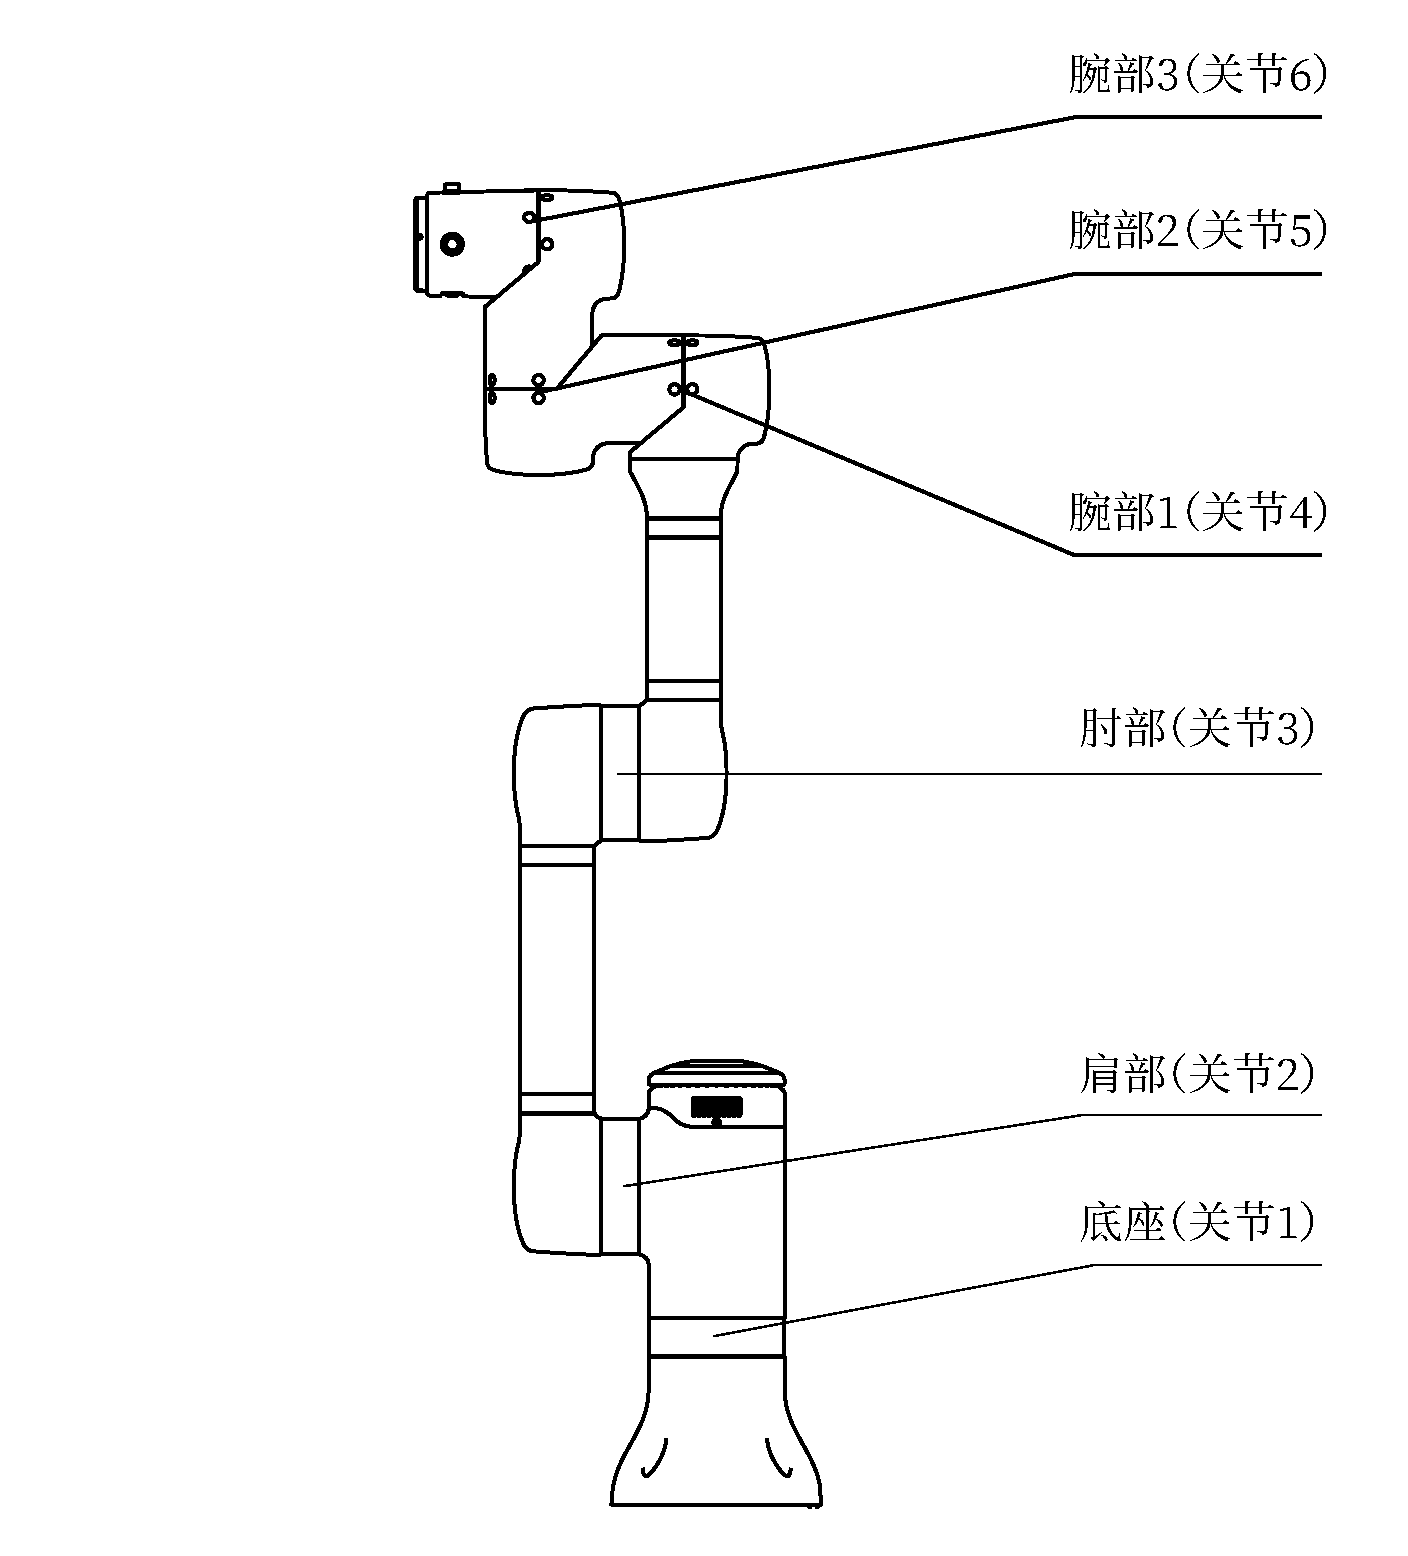
\includegraphics[height=11cm]{image/arms.pdf}
    \caption{机器人关节示意图}
    \label{fig:机器人关节示意图}
\end{figure}

机器人本体为机器人产品的执行机构(以下简称机器人),其中底座为机器人安装处,肩部和肘部可执行较大幅度动作,腕部1和腕部 2可执行较精细动作,腕部 3 可以连接末端工具。

\clearpage

控制箱为机器人系统的控制部分,可控制机器人在工作空间中的位置、姿态,连接设备的电气输入和输出端以及查看机器人的各种状态数据和信息。在实际应用场景下,为确保运行安全,通常需要在控制箱上外接急停开关(选配)。

如\prettyref{fig:机器人本体及控制箱连接}所示,控制箱通过机器人电缆与机器人连接。连接上电后\footnote{请参考\prettyref{cha:基础操作}相关内容。},用户可通过电脑、平板、手机或其他图形化终端设备的浏览器\footnote{建议使用 Google Chrome 浏览器、Microsoft Edge浏览器或其他基于Webkit 内核的现代浏览器来获得更好的体验。 }访问机器人的\LM\footnote{\LM 是本公司为机器人量身定制的机器人控制系统,所有对机器人的可视化操作和控制必须通过登录\LM 系统后再进行。}系统控制机器人。

\begin{figure}[h!]
    \centering
    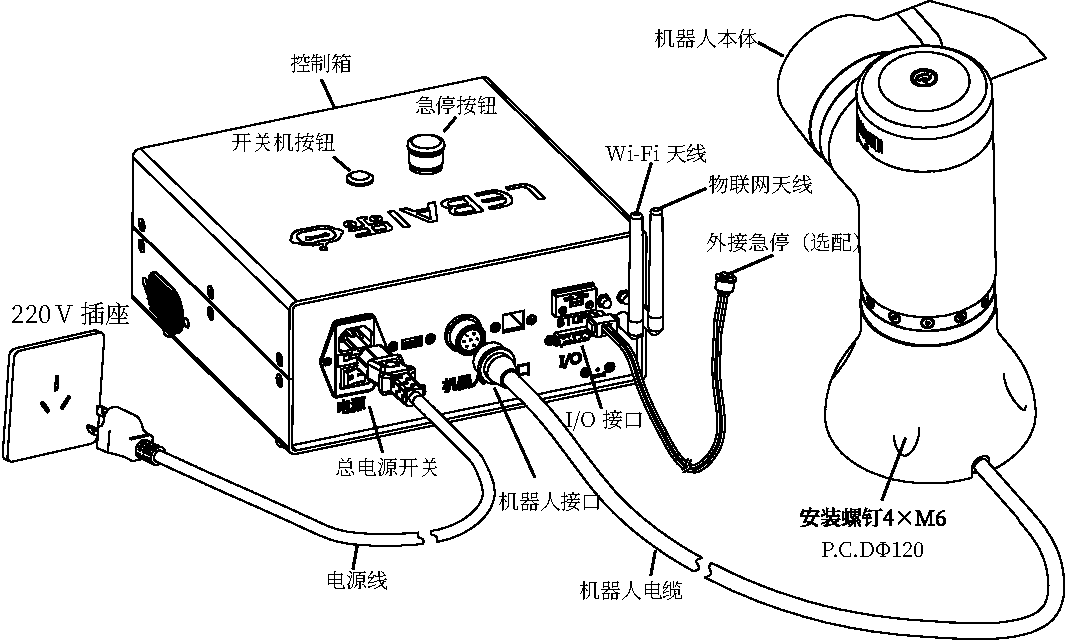
\includegraphics[width=\textwidth]{line_graphs/robot_links.pdf}
    \caption{机器人及控制箱连接}
    \label{fig:机器人本体及控制箱连接}
\end{figure}

\clearpage

\subsection{基础参数}

% 见\prettyref{tab:基础参数}。

% \begin{table}[htb!]
%     \centering
%     \rowcolors{1}{trEven}{trOdd}
%     \newcommand\Thr[1]{\cellcolor{th}\sffamily\color{white}{#1}}
%     \begin{tabular}{cllll}
% \tO & \Thr{自由度} & 6 & \Thr{工作半径} &		$638\mm $ \\
% \tO & \Thr{有效负载   } &	$\le 3\kg$ & \Thr{重量   } &	$9.5\kg$\\
% \tO & \Thr{重复精度   } &	$\pm 0.5\mm$ & \Thr{末端速度   } &	$\le 2\unit{m/s}$\\
% \tO & \Thr{环境湿度   } &	$25\sim 85\%$(无冷凝) & \Thr{环境温度} &	$0\sim 40\oC$\\
% \tO & \Thr{防护等级} &	IP54 & \Thr{供电电源} &	$48\unit{V}$(DC)\\
% \multirow{-6}{4em}{\tO 机器人} & \Thr{安装方式   } &	正装、倒装、侧装 & \Thr{安装面积   } &	$\approx 160 \unit{cm^2}$\\
% \tE & \Thr{尺寸} & $270\times 250\times 130(H) \mm$ & \Thr{重量} & $3.8\kg$ \\
% \tE & \Thr{机器人电缆长度} & $2\unit{m}$ & \Thr{供电电源} & $100\sim 240\unit{V}$(AC), $50\sim 60\unit{Hz}$ \\
% \multirow{-3}{4em}{\tE 控制箱} & \Thr{防护等级} & IP20 & \Thr{通讯协议} & 以太网  \\
%     \end{tabular} 
% \footnotesize{控制箱和机器人整机典型功耗	$150\unit{W}$}
%     \caption{乐白机器人基础参数}
%     \label{tab:基础参数}
% \end{table}

\begin{table}[htb!]
    \centering
    \rowcolors{1}{trOdd}{trEven}
    \caption{机器人基础参数}
    \label{tab:机器人基础参数}
    \begin{tabular}{m{4.2em}m{12em}m{4.2em}m{4.5em}}
\Thr{自由度} & 6 & \Thr{工作半径} &		$638\mm $ \\
\Thr{有效负载   } &	$\le 3\kg$ & \Thr{重量   } &	$9.5\kg$\\
\Thr{重复精度   } &	$\pm 0.5\mm$ & \Thr{末端速度   } &	$\le 2\unit{m/s}$\\
\Thr{环境湿度   } &	$25\!\sim\! 85\%$(无冷凝) & \Thr{环境温度} &	$0\!\sim\! 40\oC$\\
\Thr{防护等级} &	IP54 & \Thr{供电电源} &	$48\unit{V}$(DC)\\
\Thr{安装方式   } &	正装、倒装、侧装 & \Thr{安装面积   } &	$\approx 160 \unit{cm^2}$\\
    \end{tabular}

    \caption{控制箱基础参数}
    \label{tab:控制箱基础参数}
    \begin{tabular}{m{4.2em}m{12em}m{4.2em}m{4.5em}}    
\Thr{尺寸} & $270\times 250\times 130(H) \mm$ & \Thr{重量} & $3.8\kg$ \\
\Thr{供电电源} & $100\!\sim\! 240\unit{V}$(AC), $50\!\sim\! 60\unit{Hz}$ & \Thr{电缆长度} & $2\unit{m}$ \\
\Thr{防护等级} & IP20 & \Thr{通讯协议} & 以太网  \\
    \end{tabular}

\tablenote{控制箱和机器人整机典型功耗	$150\unit{W}$}
\end{table}

\vfill

\clearpage

\begin{figure}[htb!]
	\centering
	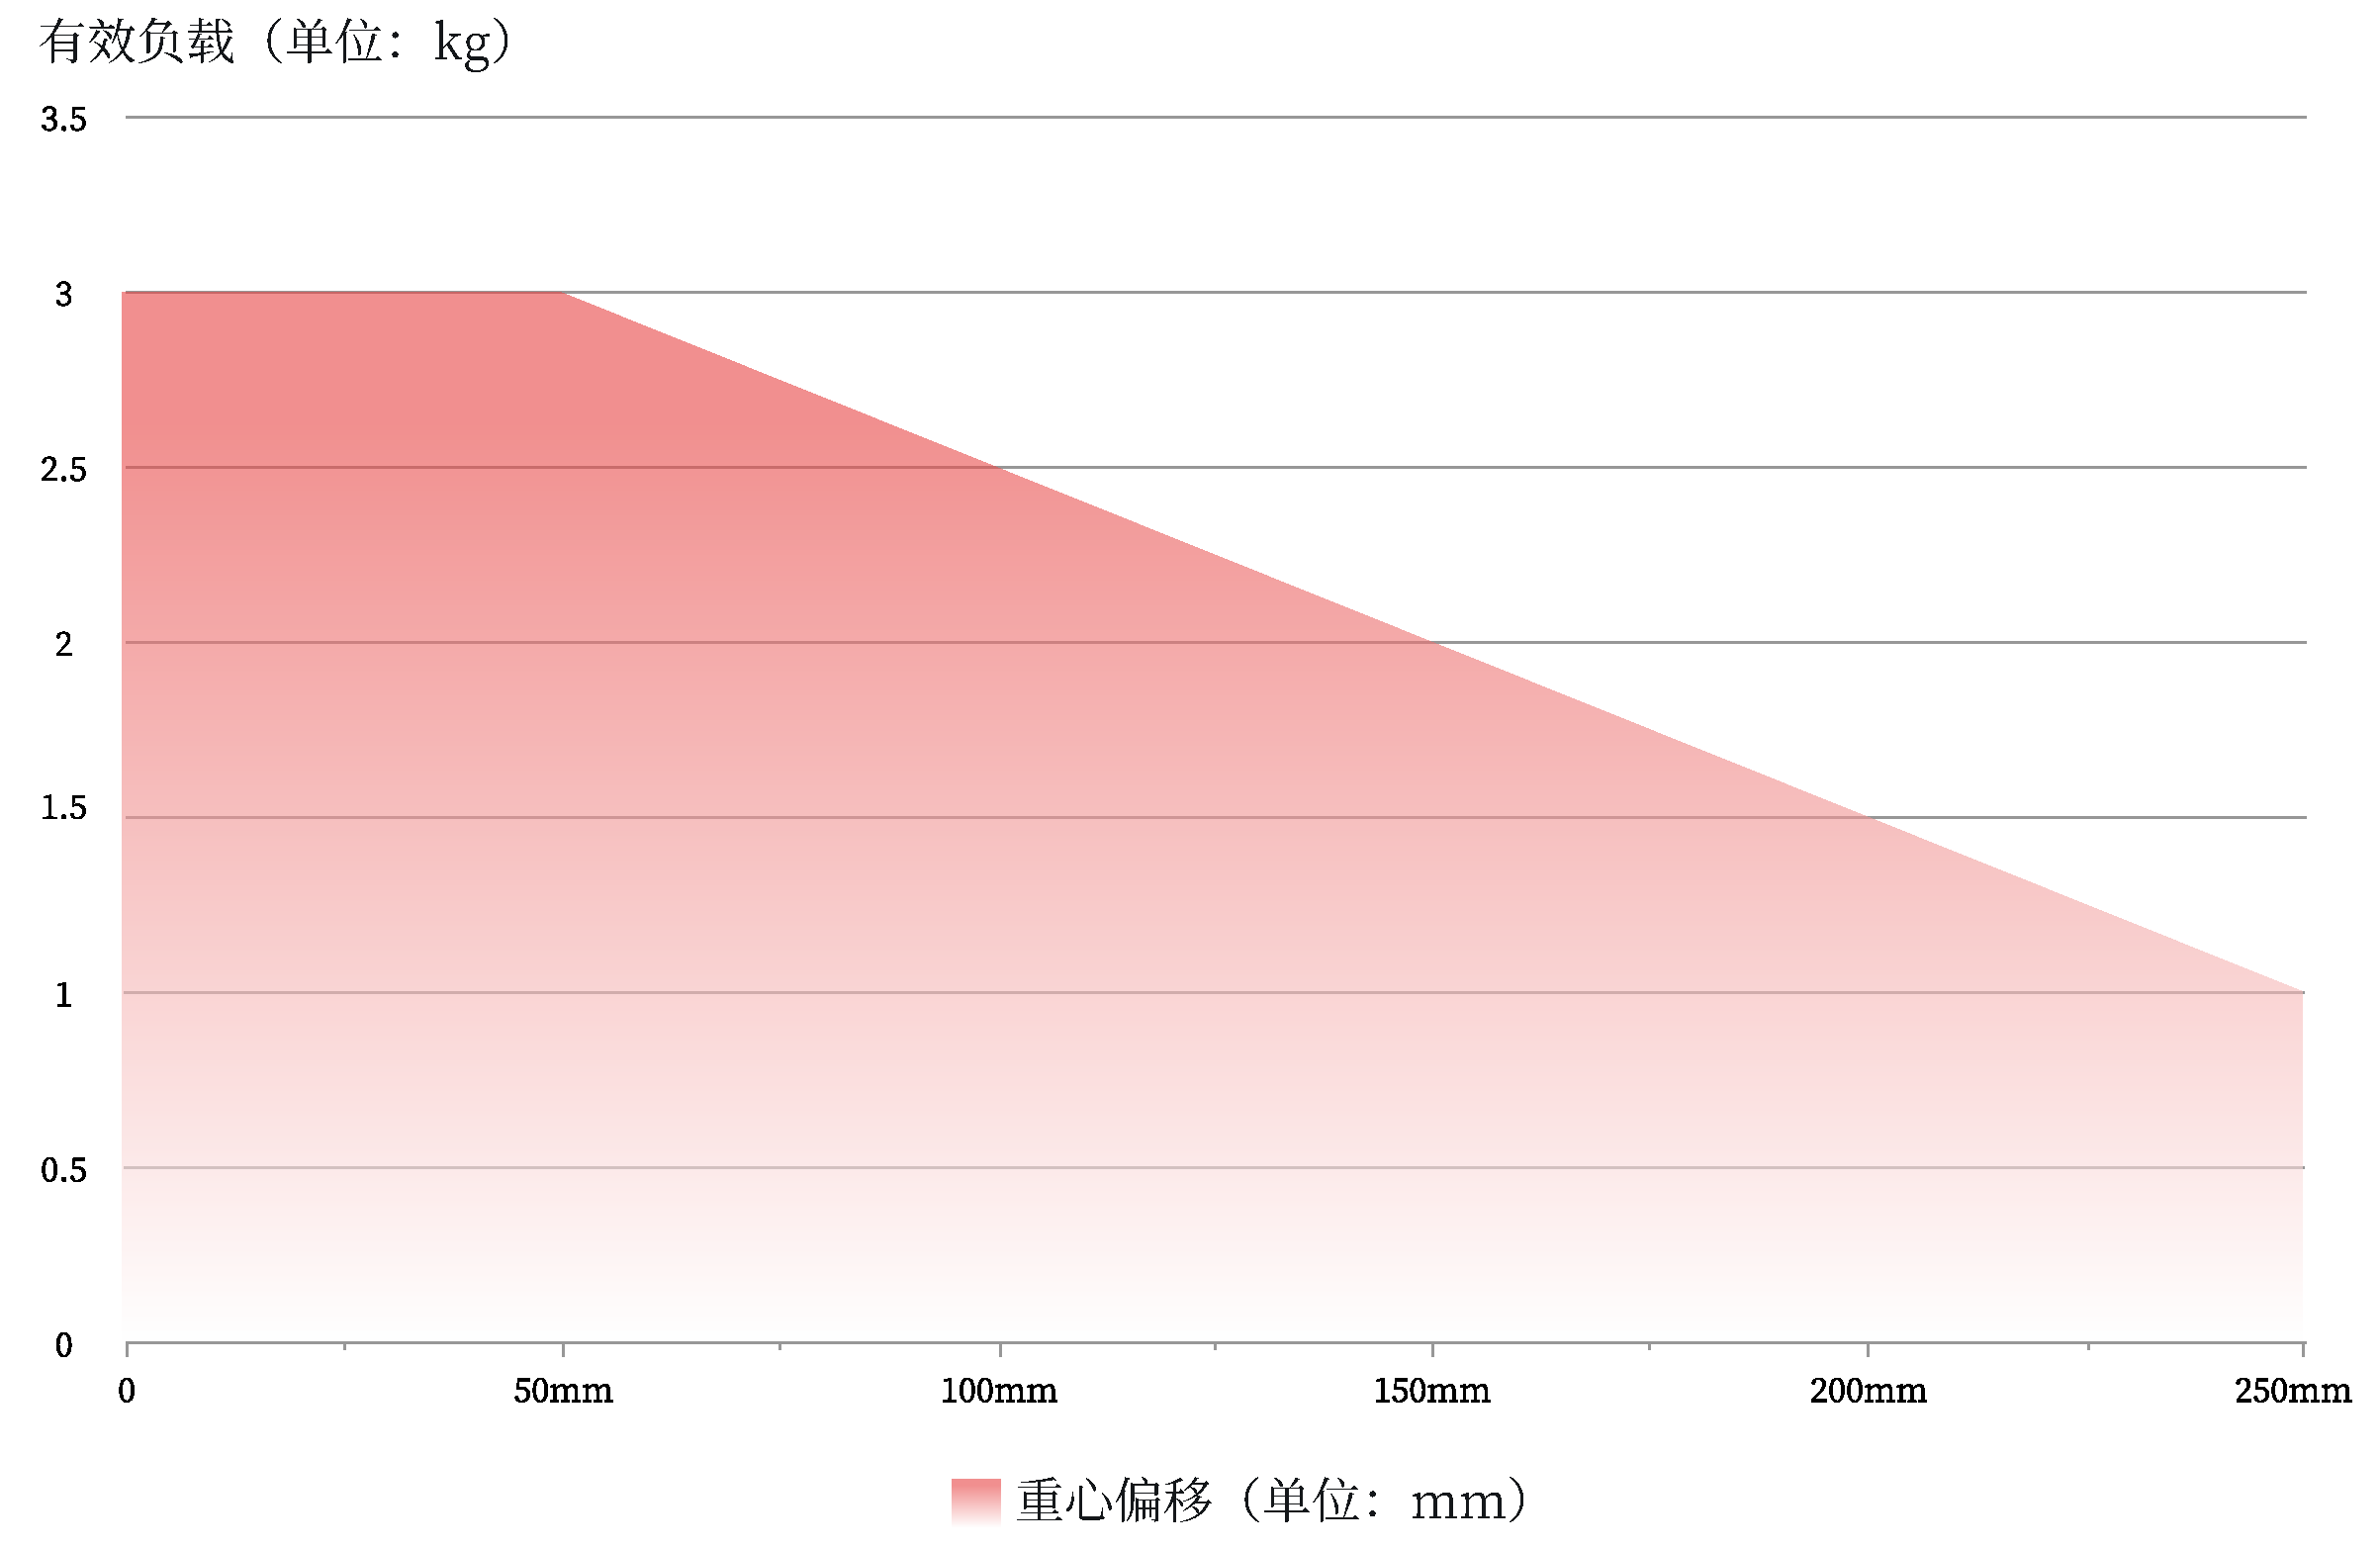
\includegraphics[width=\textwidth]{line_graphs/effective_payload.pdf}
	\caption{有效负载图}
	\label{fig:有效负载图}
\end{figure}


机器人最大允许有效负载取决于重心偏移,如\prettyref{fig:有效负载图}。重心偏移定义为工具输出法兰的中心与重心之间的距离。

\danger[警告]{\begin{itemize}
	\item 负载条件应在图表所示范围内;
	\item 图中显示的有效负载表示的是最大负载能力,在任何情况下,都不应该超过图中所示的最大重量;
	\item 超过允许值会导致机器内部件的提早损坏。
\end{itemize}}

% \clearpage

\subsection{运动轴}

% 见\prettyref{tab:运动轴}。

\begin{table}[ht]
    \centering
    \rowcolors{1}{trEven}{trOdd}
    \def\dps{\unit{^\circ/s}}
    \caption{乐白机器人运动轴}
    \label{tab:运动轴}
    \begin{tabular}{ccc}
\rowcolor{th} \Th{关节} &	\Th{运动范围} &	\Th{最大速度}\\
关节1   &	无限制  &	$180\dps$ \\
关节2   &	无限制  &	$180\dps$ \\
关节3   &	无限制  &	$180\dps$ \\
关节4   &	无限制  &	$180\dps$ \\
关节5   &	无限制  &	$180\dps$ \\
关节6   &	无限制  &	$180\dps$ \\
    \end{tabular}

    \tablenote{以上所提的关节运动范围无限制需排除机器人自干涉的情况,\\
    自干涉的情况因实际运动场景而有差异}
\end{table}

\clearpage

\subsection{工作空间}

% 见\prettyref{fig:机器人运动范围}。

\begin{figure}[ht]
    \centering
    \subfigure[沿$Z$轴方向]{
    	\begin{minipage}[b]{0.4\textwidth}\centering
   		 	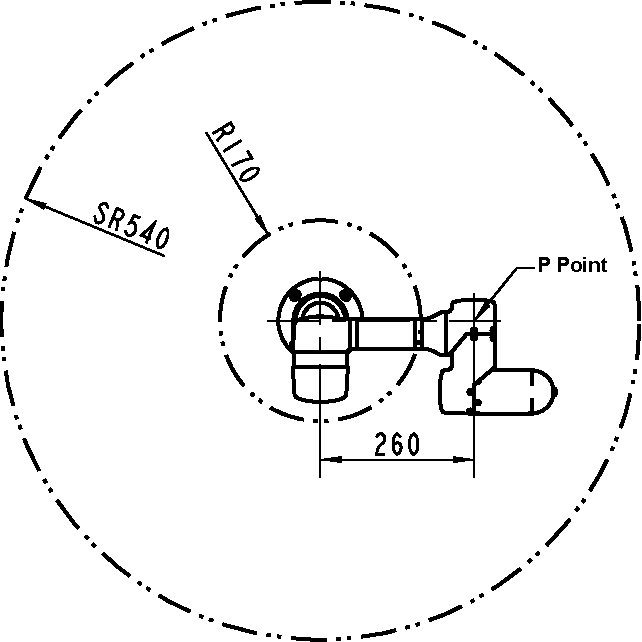
\includegraphics[width=\linewidth]{line_graphs/view-via-z.pdf}
    	\end{minipage}
    }
    \subfigure[沿$X$轴或$Y$轴方向]{
    	\begin{minipage}[b]{0.4\textwidth}\centering
   		 	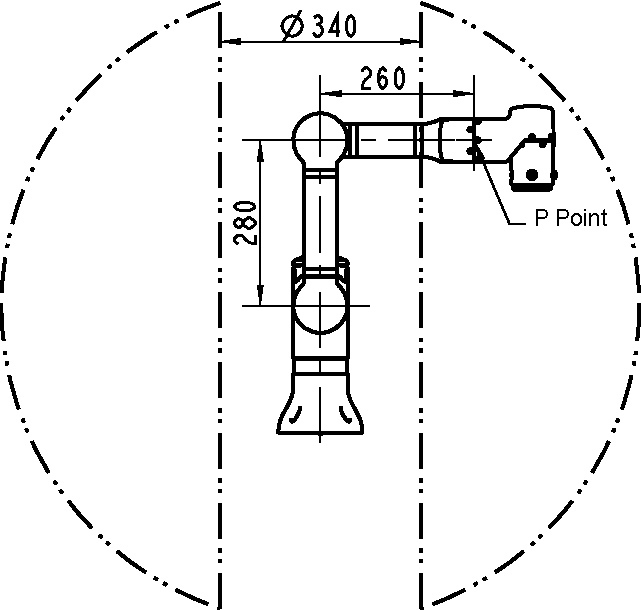
\includegraphics[width=\linewidth]{line_graphs/view-via-xy.pdf}
    	\end{minipage}
    }
    \caption{乐白机器人工作空间示意图}
    \label{fig:机器人运动范围}
\end{figure}

% \clearpage

\subsection{I/O接口}

LM3提供的I/O接口有两部分:控制箱和末端法兰盘,根据不同的应用场景,您可以选择不同位置的I/O接口来实现相应的I/O操作。

\begin{enumerate}
    \item 如\prettyref{fig:控制箱IO}和\prettyref{tab:控制箱IO},机器人控制箱提供:
    \begin{itemize}
        \item 4个数字输入,4个数字输出接口;
        \item 2个模拟输入,2个模拟输出接口。
    \end{itemize}

\begin{table}[htb!]
    \centering
    % \rowcolors{1}{trEven}{trOdd}
\begin{tabular}{cll}
\rowcolor{th} \Th{序号}	&  \Th{功能}	& \Th{性能参数}\\
\tO  1	& \tO 电源正极	& \tO $24\unit{V}$  \\
\tE  2	& \tE 模拟输出1 & \tE \\
\tO  3	& \tO 模拟输出2 & \multirow{-2}{5cm}{\tE 电压型:输出电压$0\sim 10\unit{V}$\\电流型:输出电流$4\sim 20\unit{mA}$}\\
\tE  4	& \tE 数字输出1	& \tO \\
\tO  5	& \tO 数字输出2	& \tO \\
\tE  6	& \tE 数字输出3	& \tO \\
\tO  7	& \tO 数字输出4	& \multirow{-4}{5cm}{\tO 输出电压$24\unit{V}$,最大电流$2\unit{A}$}\\
\tE  8	& \tE 电源负极	& \tE \\
\tO  9	& \tO 模拟输入1 & \tO \\
\tE  10	& \tE 模拟输入2	& \multirow{-2}{5cm}{\tO 电压型:输出电压$0\sim 10\unit{V}$\\电流型:输出电流$4\sim 20\unit{mA}$    }\\
\tO  11	& \tO 数字输入1	& \tE \\
\tE  12	& \tE 数字输入2	& \tE \\
\tO  13	& \tO 数字输入3	& \tE \\
\tE  14	& \tE 数字输入4	& \multirow{-4}{5cm}{\tE 输入电压$3\sim 30\unit{V}$}\\
\tO  15	& \tO 电源负极	& \tO \\
% \tE GND & \tE & \tE \\
\end{tabular}
\caption{控制箱I/O接口引脚说明}
\label{tab:控制箱IO}
\end{table}

    \item 如\prettyref{fig:法兰盘IO}和\prettyref{tab:法兰盘IO},末端法兰盘上提供:
    \begin{itemize}
        \item 2个数字输入接口;
        \item 2个数字输出接口。
    \end{itemize}

\begin{figure}[htb!]
    \centering
    \includegraphics[height=3cm]{line_graphs/robot_box_io_plugin.pdf}
    \caption{控制箱I/O硬件接口示意图}
    \label{fig:控制箱IO}
\end{figure}

\begin{figure}[htb!]
    \centering
    \includegraphics[height=2cm]{image/35.pdf}
    \caption{末端法兰盘 I/O硬件接口示意图}
    \label{fig:法兰盘IO}
\end{figure}

\begin{table}[htb!]
    \centering
    \rowcolors{1}{trEven}{trOdd}
    \def\tE{\cellcolor{trEven}}
    \def\tO{\cellcolor{trOdd}}
\begin{tabular}{cll}
   \rowcolor{th}\Th{序号}	&  \Th{功能}	& \Th{性能参数}\\
    1	&   电源正极 & \tO \\
    2	&   电源负极 & \multirow{-2}{5cm}{\tO
            电压$24\unit{V}$,最大电流$2\unit{A}$    }\\
    3	&   数字输出1	&  \tE \\
    4	&   数字输出2	&   \multirow{-2}{5cm}{\tE 输出电压$24\unit{V}$,最大电流$2\unit{A}$}\\
    5	&   CANH	&  CAN通信总线高电平 \\
    6	&   CANL	& CAN通信总线低电平  \\
    7	&   数字输入1	&  \tO \\
    8	&   数字输入2	&  \multirow{-2}{5cm}{\tO
            输入电压$3\sim 30\unit{V}$
    } \\
\end{tabular}
\caption{末端法兰盘I/O引脚说明}
\label{tab:法兰盘IO}
\end{table}

\end{enumerate}

% \clearpage

\subsection{网络连接}

LM3提供以太网、Wi-Fi(2.4 GHz) 热点网络、4G物联网三种网络连接方式。其中:以太网和Wi-Fi网络连接用于提供给用户操作和连接机器人使用,4G物联网连接目前仅用于设备基础信息\footnote{设备基础信息仅限于:设备名称,设备网络连接类型及状态,软件系统版本,系统运行错误信息且不包含任何客户业务数据(包括且不限于场景数据等)。如需其他信息的上报,乐白将事前获得您的授权同意后才进行。}的数据上报。

% \vfill

% \clearpage

\section{机器人安装}

如\prettyref{fig:机器人安装方式},LM3机器人支持三种安装方式:正装、倒装、侧装(侧装时注意机器人电缆出口必须朝下)。

\begin{figure}[ht]
    \centering
    \subfigure[正装]{
		\begin{minipage}[b]{0.3\textwidth}\centering
			\includegraphics[width=\linewidth]{line_graphs/install_direction_up.pdf}
		\end{minipage}
	}
    \subfigure[倒装]{
    	\begin{minipage}[b]{0.3\textwidth}\centering
   		 	\includegraphics[width=\linewidth]{line_graphs/install_direction_down.pdf}
    	\end{minipage}
    }
    \subfigure[侧装]{
    	\begin{minipage}[b]{0.3\textwidth}\centering
   		 	\includegraphics[width=\linewidth]{line_graphs/install_direction_side.pdf}
    	\end{minipage}
    }
    \caption{机器人安装方式}
    \label{fig:机器人安装方式}
\end{figure}

% \clearpage

\begin{figure}[ht]
    \centering
    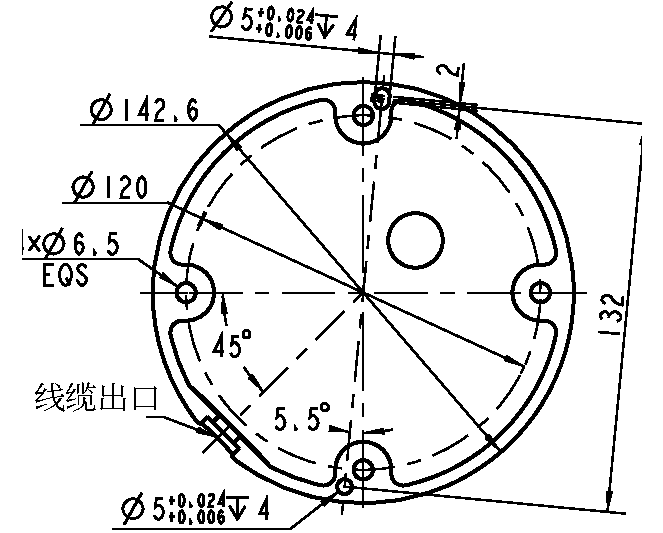
\includegraphics[height=5cm]{line_graphs/bottom_surface.pdf}
    \caption{机器人底座视图}
    \label{fig:机器人底座视图}
\end{figure}

使用机器人配件包中的 4 颗 M6 螺钉,对应机器人底座(如\prettyref{fig:机器人底座视图})上的 4 个安装孔进行安装操作,建议以 $9\Nm$ 扭矩紧固这些螺钉。如果需要更准确地调整机器人位置,还可钻2 个直径$5 \mm$的孔,并用销加以固定。

\info{\begin{itemize}
\item 机器人每一个安装孔位都应固定螺钉,固定后的每个螺钉都应能提供最小抗倾覆力;
\item 机器人安装时,应扶住机器人直至底座所有螺钉全部紧固好。
\end{itemize}}

\danger[警告]{切勿将机器人(含控制箱)固定在不稳固的位置,否则可能会跌落损坏。}

\chapter{基础操作}
\label{cha:基础操作}

\section{机器人上电}

操作前,请再次确认已阅读并确保已遵循\prettyref{sec:安全指南}内容,排除潜在风险,确保操作安全。

\begin{figure}[hb]
    \centering
    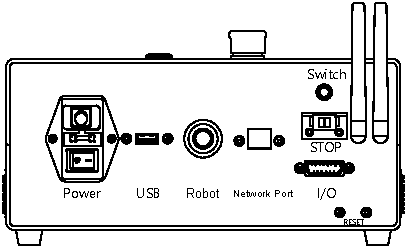
\includegraphics[height=4cm]{line_graphs/robot_control_box_back.pdf}
    \caption{控制箱背板示意图}
    \label{fig:控制箱背板示意图}
\end{figure}

\begin{enumerate}
\item 将机器人电缆插头插入控制箱的机器人接口;
\item 控制箱插上电源线,并将电源插头接入$220 \unit{V}$交流电插座;
\item 确保控制箱顶部的急停按钮处于释放\footnote{当机器按钮处于弹起状态时为释放状态,反之处于按下状态为锁定状态。}状态;
\item 打开控制箱背板的红色总电源开关,开关指示灯亮;
\item 长按控制箱顶部的开关机按钮(约3 秒),直至蓝色灯光常亮,等待机器人肩部灯光亮起,完成控制箱和机器人的上电操作。
\end{enumerate}

\danger{\begin{itemize}
\item 请确保控制箱电源的插线板务必良好接地;
\item 请确保控制箱电源的输入电流受到漏电保护装置和适当的过流断路保护装置的保护;
\item 请确保所有的电缆在控制箱通电前都正确连接,始终正确使用原装的电源线。
\end{itemize}}

\danger[警告]{\begin{itemize}
\item 禁止在机器人启动时断开或用力拉拽机器人电缆;
\item 禁止延长或改动机器人电缆;
\item 切勿损坏电源线,或将重物压在电源线上;
\item 切勿使用破损或不符合的插座。
\item 切勿让电源插头和插座粘附灰尘和金属附着物。
\end{itemize}}

\clearpage

\section{连接机器人}
LM3支持有线网络连接和无线网络连接,无线网络连接目前仅支持接入控制箱内置的Wi-Fi热点网络。
\subsection{有线网络连接}

使用网线将控制箱背板的网口与路由器或交换机连接,同时确保用于操作机器人的电脑、平板、手机或其他图形化终端设备与机器人接入的是同一网络。

有线网络的连接示意如\prettyref{fig:有线网络连接拓扑图}:

\begin{figure}[ht]
    \centering
    \includegraphics[width=\textwidth]{image/1103/5.pdf}
    \caption{有线网络连接拓扑图}
    \label{fig:有线网络连接拓扑图}
\end{figure}

\clearpage

\subsection{无线网络连接}
机器人出厂后,默认会启用一个热点名称为设备名称  的Wi-Fi热点,设备名称格式如:\verb|Lebai-123456|(后6位为随机字符),默认密码为:\verb|88888888|(8个8)。可通过电脑、平板、手机或其他图形化终端设备的Wi-Fi功能连接该设备名称对应的Wi-Fi热点网络,连接和控制机器人。

\begin{figure}[ht]
    \centering
    \includegraphics[width=\textwidth]{image/12.pdf}
    \caption{无线网络连接拓扑图}
    \label{fig:无线网络连接拓扑图}
\end{figure}

\clearpage

\section{登录\LM}
熟悉\LM 系统的操作将有助于您更方便和快速地上手使用本公司的机器人产品。
打开电脑、平板、手机或其他图形化终端设备的浏览器,在地址栏输入如下地址:
\begin{itemize}
	\item 若使用有线网络,地址\footnote{有线网络地址在接入的网络路由器页面中的设备列表里查看,查看方式因设备品牌和类型的不同而有差异,具体查看方式请参考路由器设备的说明书或联系对应设备厂商。}为:\url{http://<IP>}
	\item 若使用无线热点,地址为:\url{http://10.20.17.1}
\end{itemize}

网页打开后会进入登录页面,请输入默认授权码:\verb|1111|,点击\btn{登录}或按\kbd{Enter},登录\LM。

\begin{figure}[ht]
    \centering
    \includegraphics[width=0.8\textwidth]{screen/2-4.png}
    \caption{登录\LM}
    \label{fig:登录LM}
\end{figure}

\clearpage

\section{设置引导页}

当机器人开箱上电后,第一次登录\LM 时,首先需要按照设置引导页的提示进行初次使用的安装设置。
\subsection{系统设置}
在此步可以自定义语言、时区、时间。

\begin{figure}[ht]
    \centering
    \includegraphics[width=\textwidth]{screen/2-5.png}
    \caption{系统设置}
    \label{fig:系统设置}
\end{figure}

\subsection{机器人设置}
在此步中可以设置机器人的安装方式、操作模式及碰撞检测。
\begin{enumerate}
\item 安装方式

	根据实际安装方式,参照\prettyref{fig:安装方式}中的“图标对照表”选择正装、倒装、侧装。

	\begin{figure}[ht]
		\centering
		\includegraphics[width=\textwidth]{screen/2-6.png}
		\caption{安装方式}
		\label{fig:安装方式}
	\end{figure}

	\danger{安装方式的选择一定要与实际安装方式一致,否则有可能导致误伤。}

\clearpage

\item 操作模式

	可在新手模式、专家模式中选择。新手模式适合没有编程基础的新手,无需理解任何逻辑和代码;专家模式适合有一定编程基础和逻辑基础的高级用户,您可以根据自身情况选择相应的操作模式。

	\begin{figure}[ht]
		\centering
		\includegraphics[width=\textwidth]{screen/2-7.png}
		\caption{操作模式}
		\label{fig:操作模式}
	\end{figure}

\clearpage

\item 碰撞检测

	检测开关默认为开,“碰撞后的动作”默认为\mnu{急停},可选择\mnu{急停}或\mnu{暂停},同时可以拖动拉杆来调整“检测灵敏度”大小。点击\btn{下一步},进入界面设置。

	\begin{figure}[ht]
		\centering
		\includegraphics[width=\textwidth]{screen/2-8.png}
		\caption{碰撞检测}
		\label{fig:碰撞检测}
	\end{figure}

	\danger{机器人运行过程中,无论是否开启“碰撞检测”功能,禁止在没有防护的情况下进入到机器人作业半径范围内,否则存在人员被机器人撞伤,卷入的危险。}

\end{enumerate}

\clearpage

\subsection{界面设置}

在界面设置中,建议您选择使用\mnu{深色主题}。
% 可以选择\mnu{深色主题}或\mnu{浅色主题},目前\LM 浅色主题还在测试阶段,

\begin{figure}[ht]
	\centering
	\includegraphics[width=\textwidth]{screen/2-9.png}
	\caption{界面设置}
	\label{fig:界面设置}
\end{figure}

点击\btn{完成},进入\LM 首页。

\clearpage

\section{首页}

在\LM 首页,页面分为:左面板、状态区、控制区、主功能入口、任务历史以及顶部标题栏六个区域。

左面板显示机器人整机温度及关节温度数据,坐标空间的位置和姿态数据,关节空间的关节角度数据;状态区显示机器人的实时状态;控制区包含机器人的启停按钮,软件示教按钮以及速度比例调整控件;主功能入口包含场景、控制和设备三个主功能入口;任务历史包含所有的任务历史列表;顶部标题栏右侧包含设置、消息中心和退出登录。

\begin{figure}[ht]
	\centering
	\includegraphics[width=\textwidth]{screen/2-10.png}
	\caption{\LM 首页}
	\label{fig:LM首页}
\end{figure}

\clearpage

\subsection{机器人状态}

机器人状态区显示机器人当前状态,具体说明可参考\prettyref{tab:机器人状态列表}。

\begin{table}[ht]
    \centering\small
    \begin{tabular}{|l|l|}\hline
\sf 状态 & \sf 说明\\\hline
硬件通讯故障 & 机器人通讯故障或控制系统异常\\\hline
已急停,请确认安全性 & 机器人处于急停状态\\\hline
初始化中 & 机器人初始化中\\\hline
初始化完成 & 机器人电源已开启\\\hline
空闲 & 机器人处于空闲状态\\\hline
运行中 & 机器人运行中\\\hline
更新中 & 机器人系统更新中\\\hline
启动中 & 机器人初始化完成到空闲的启动过程中\\\hline
正在停止 & 机器人空闲状态转到停止状态\\\hline
示教中 & 机器人处于示教模式中\\\hline
已停止 & 机器人处于停止状态,非急停状态\\\hline
    \end{tabular}
    \caption{机器人状态列表}
    \label{tab:机器人状态列表}
\end{table}

\subsection{温度}
如\prettyref{fig:温度信息},\LM 首页左上方实时监测机器人整机温度\footnote{整机温度:取控制箱内控制器的CPU温度和机器人每个关节的温度的最大值作为整机温度的显示,当整机温度数值右侧显示芯片图标为表示当前CPU温度值最高,显示一个关节加数字图标时表示该数字对应的关节温度较高。},每个关节正常温度范围值在室温至65 ℃之间。点击左边区域的关节空间标签中关节角度的右侧温度计图标,可实时观测关节1至关节6的温度变化;再次点击该图标,可以切换回关节角度显示。

\danger[警告]{当关节温度显示超过65℃时,请勿触摸机器外表面,否则有高温烫伤风险,并请立即停机,待机器温度回到常温,再检查当前机器人负载是否超过额定有效负载$3\kg$或者机器人是否碰撞到外部物品。}

\begin{figure}[ht]
	\centering
	\begin{minipage}[t]{0.32\linewidth}
		\centering
		\includegraphics[height=6cm]{screen/2-11-t.jpg}
		\caption{关节温度}
		\label{fig:温度信息}
	\end{minipage}
	\begin{minipage}[t]{0.32\linewidth}
		\centering
		\includegraphics[height=6cm]{screen/2-12-1.png}
		\caption{关节空间}
		\label{fig:关节位置信息}
	\end{minipage}
	\begin{minipage}[t]{0.32\linewidth}
		\centering
		\includegraphics[height=6cm]{screen/2-12.png}
		\caption{坐标空间}
		\label{fig:坐标位置信息}
	\end{minipage}
\end{figure}

\subsection{位置信息}
\LM 首页左侧区域实时同步机器人位置信息,包含坐标空间和关节空间。如\prettyref{fig:坐标位置信息},坐标空间显示机器人在坐标空间的位置和姿态的实时数据;如\prettyref{fig:关节位置信息},关节空间显示机器人6个关节角度的实时数据。

\subsection{速度因子}
点击\LM 首页示教按钮下方的速度图标,在展开的滑动条中拖动滑块或点击滑动条以调整机器人的运行速度比例,调整区间为$0\sim 100$。

\begin{figure}[ht]
	\centering
	\includegraphics[height=4cm]{screen/2-13.png}
	\caption{速度因子}
	\label{fig:速度因子}
\end{figure}

\subsection{消息中心}
在消息中心中,可查看机器人提示、警告、软硬件异常的消息通知。鼠标移动到\LM 首页右上角的消息图标\icn[Black]{image/22.pdf}可以打开消息中心。

在消息中心中,有以下两种方式进行消息搜索:
\begin{enumerate}
	\item 通过关键字搜索消息通知;
	\item 通过筛选5种类型的机器人消息通知:
	\begin{description}
\item[\icn{image/30.pdf} 调试]
\item[\icn{image/29.pdf} 信息] 信息提醒类消息
\item[\icn{image/28.pdf} 警告] 系统运行时的警告级别的提醒,一般不影响使用
\item[\icn{image/27.pdf} 错误] 系统出现了错误,需要保持关注错误的发生概率,如果频繁发生需尽快点击查看解决方案或与本公司及时取得联系
\item[\icn{image/26.pdf} 致命] 系统出现严重错误,存在运行风险或已无法正常运行,此时必须立即停机查看解决方案或与本公司及时取得联系。
	\end{description}
\end{enumerate}

点击消息项的错误码链接,可跳转至本公司官网对应的错误码解决方案查看页面,在页面中可根据错误码查找对应的问题及解决方案。

\subsection{任务历史}
\label{sec:任务历史}
任务历史列表中显示正在运行中及已完成的任务,并以时间顺序排列展现。当任务正在运行时,任务历史标题栏会出现停止、暂停或恢复的控制按键。任务历史列表中:
\begin{itemize}
	\item 正在运行的任务右侧显示当前已运行次数;
	\item 已完成的任务右侧显示“重新运行”小旗帜\icn{image/38},点击可重新运行当前选择的任务。
\end{itemize}

点击“任务历史”列表项任务名称,进入该任务对应的场景编辑页面。

\danger[警告]{当运行某个场景,该场景的任务进入任务历史列表。该任务运行完成,点击“重新运行”按钮后,当前执行的任务为之前执行该任务的场景数据,即使该场景在该任务运行完后发生变更,也不会影响该任务的重新运行,重新运行的任务不受该场景的数据变更影响,以上一次运行任务的场景数据为准。}

\begin{figure}[htb]
	\centering
	\begin{minipage}[t]{0.55\linewidth}
		\centering
		\includegraphics[height=8cm]{screen/2-14.png}
		\caption{消息中心}
		\label{fig:消息中心}
	\end{minipage}
	\hfill
	\begin{minipage}[t]{0.4\linewidth}
		\centering
		\includegraphics[height=8cm]{screen/2-15.png}
		\caption{任务历史}
		\label{fig:任务历史}
	\end{minipage}
\end{figure}

\clearpage

\section{启动机器人}
进入\LM ,如\prettyref{fig:启动机器人}所示,点击首页蓝色启动按钮\icn{image/39.pdf};当首页视图区上方机器人状态标签显示为\mnu{空闲}时,表示您已成功启动机器人。

\begin{figure}[ht]
	\centering
	\includegraphics[width=\textwidth]{screen/2-16.png}
	\caption{启动机器人}
	\label{fig:启动机器人}
\end{figure}

\section{停止机器人}
当机器人处于\mnu{运行中}或\mnu{空闲}状态时,可以点击首页或如\prettyref{fig:胶囊控制区}所示的胶囊控制区的红色停止按钮;当机器人状态变为\mnu{已停止}时,表示您已成功停止机器人。

% \begin{figure}[ht]
% 	\centering
% 	\includegraphics[width=\textwidth]{image/6.pdf}
% 	\caption{\LM  首页--停止机器人}
% 	\label{fig:停止机器人}
% \end{figure}

\section{急停机器人}

急停操作有两种方式,可任选其一:
\begin{description}
	\item[软急停] \LM 右下方的红色\btn[Danger]{急停ESTOP}按钮;
	\item[硬急停] 按下控制箱顶部的红色凸起急停按钮或外接急停按钮(选配)。
\end{description}

\info{使用硬急停操作后,急停操作不会自动释放,需要顺时针旋转急停按钮,解除锁定后完成释放。}

\section{关闭机器人}
\begin{enumerate}
	\item 先停止或者急停机器人;
	\item 长按控制箱开关机按钮,直至蓝色灯光熄灭;
	\item 关闭控制箱背板的红色总电源开关。
\end{enumerate}

\danger[警告]{关闭机器人需严格遵守上述操作步骤,否则可能导致机器人文件系统损坏、机器人功能故障等问题。}

\section{胶囊控制区}
胶囊控制区仅在非首页时显示,可查看“机器状态”和“任务历史”。长按可拖动调整胶囊控制区在页面中的位置。

\begin{figure}[hb]
	\centering
	\includegraphics[height=4cm]{screen/2-18.png}
	\caption{胶囊控制区}
	\label{fig:胶囊控制区}
\end{figure}

\begin{description}
	\item [机器状态] 包含机器人当前状态、机器人启动/停止按钮、示教按钮以及速度调整拉杆,可以在非首页时操作和控制机器人;
	\item [任务历史] 包含正在运行中及已完成的任务列表、任务的暂停/恢复和停止按钮,可以在非首页时查看任务历史,具体操作见\prettyref{sec:任务历史}。
\end{description}

\chapter{使用机器人}

场景为操作和使用机器人的基本功能模块,编写一个新场景即可开始操作机器人。在讲述如何创建和编写一个场景之前,我们先介绍下乐白机器人的场景编辑器以及如何进行拖动示教 操作。
场景编辑器
编辑器类型
乐白机器人场景编辑操作支持使用如下两种编辑器进行编辑:
时间轴编辑器
(需补充分区示意图)






图 4 1 时间轴编辑器功能分区
 可视化编辑器,低门槛无需理解任何逻辑关系,只需要按照操作说明和引导完成相应的动作块场景编写,即可让机器人运动起来。
代码编辑器


图 4 2  代码编辑器功能分区
(设计改一下lebai乐白为L MASTER)
针对高级用户,我们提供更专业的基于Lua语言的代码编辑器,使用代码编辑器可以完成各种复杂的逻辑和自定义的操作流程,可定制化程度高,需要具备一定的编程基础和逻辑基础。
切换编辑器类型
代码编辑器仅在专家模式下可用,从时间轴编辑器转换到代码编辑器的步骤如下:
	进入“设置”->“操作模式“页或点击时间轴编辑器编辑区右上角“时间轴编辑器”右边的 按钮,进入操作模式选择页,选择专家模式,点击操作模式页右上角的”保存“按钮;
	返回之前编辑的场景;
	进入时间轴编辑器,点击编辑区右上角的“时间轴编辑器”按钮,在下拉弹框中选择“代码编辑器”进行切换

图 4 3 切换编辑器类型

 	注意:
当某个场景的编辑器类型从时间轴编辑器切换成代码编辑器后,无法再将当前场景的编辑操作转换为时间轴编辑器。

类型图标说明
 在场景列表和场景编辑器页面出现此图标表示该场景为时间轴编辑器类型;
 在场景列表和场景编辑器页面出现此图标表示该场景为代码编辑器类型。

拖动示教
在讲述如何添加位置动作块之前,有必要先了解下乐白机器人的拖动示教方法。拖动示教有如下两种操作方法,可任选其一:
在L MASTER点击示教图标 使机器人进入示教状态,拖动机器人到达指定位置,再次点击示教图标,结束示教状态;
长按机器人末端凸按钮,使机器人进入示教状态,拖动机器人到达指定位置后,释放机器人末端凸按钮,结束示教状态。

 	警告:
在使用拖动示教前,请务必确保正确设置好末端设备的质量与质心,不正确的设置可能导致误伤。

 	警告:
示教过程中注意关节角度的转动不可超出安全范围,否则可能导致机器人急停或其他故障。

编写场景
创建新场景
点击L MASTER首页的场景按钮,进入场景列表,点击该页面工具栏右侧的“添加场景”按钮,输入场景名称,完成新场景的创建。

图 4 4  创建场景
使用时间轴编辑器编辑
时间轴编辑器支持的动作块类型有:
位置
手爪
等待
消息提示
数字I/O
模拟I/O
信号量
负载配置
点击时间轴编辑器任意蓝色 号图标,可以弹出选择添加动作块对话框,如图 4 5 添加动作块对话框所示。

图 4 5 添加动作块对话框
下面章节依次讲述不同动作块类型的使用方法。
位置动作块
位置控制作为机器人控制里面的核心控制模块,在时间轴编辑器中,只需要按照如下教程添加位置动作块,即可让机器人按照预定的位置动作进行相应类型的轨迹运动。
添加位置
在时间轴编辑器中添加位置有如下两种操作方法,可任选其一:
时间轴编辑器内编辑区蓝色加号(补图标)按钮,选择位置图标,在打开的添加位置对话框(如图 4 6 添加位置对话框所示)中输入位置名称,并选择蓝色“添加”字样,即可将机器人当前位置保存在一个新的位置动作块 ;
双击机器人末端凸按钮,系统将机器人当前位置保存在一个新的位置动作块。

图 4 6  添加位置对话框
通过结合拖动示教和上述添加位置动作块的方法,按照您的需求添加想要的位置动作块(可任意多个),直至场景编写完成。
编辑位置
将光标放在位置块上使当前位置块处于焦点状态,如图 4 7  位置块焦点状态所示:

图 4 7  位置块焦点状态
轨迹类型切换区的两个按钮用于切换关节空间的运动(movej)和笛卡尔空间的直线运动(movel)。
 表示关节空间 的运动;
 表示笛卡尔空间 的直线运动。
编辑操作按钮区从左至右的按钮依次为:
(每个按钮补充对应的图标,同时不带背景,上面两个轨迹类型的图标同样需更新)
样式:可以更换位置块背景颜色;
微调:对当前位置块存储的位置数据进行微调及更新;
速度及加速时间:调整位置块的速度和加速时间 ;
复制:复制一个当前的动作块;
删除:可删除当前动作块。
	微调
在场景编辑时,动作轨迹中的位置需要精准细微调整,可以对单个位置进行微调。选择微调图标,页面可自动跳转至微调页面。
微调页面中虚拟机器人和真实机器人底座重叠展示,其中虚拟机器人表示当前位置块存储的目标位置,真实机器人表示机器人当前位置。通过实际位置和目标位置切换按钮 进行切换,可查看目标位置与实际位置的数值。
	坐标空间微调

图 4 8  坐标空间微调
(添加标注)
坐标空间可选择相对于底座/末端
相对于底座时,参考坐标系可使用直角坐标系或圆柱坐标系;
相对于末端时,参考坐标系仅支持直角坐标系。

图 4 9  坐标空间示意图
参考坐标系选择“相对于底座”,就是以机器人底座平面的圆心作为世界坐标系原点,通过选择直角坐标系为调整方式,在微调页面位置信息展示框中输入位置(X, Y, Z)或姿态 (Rz, Ry, Rx)的数值,机器人会自动移动到您所需要的位置;或通过拉动屏幕下方各个方向的拉杆进行操作,当释放拉杆时,微调停止。点击“更新”按钮,完成位置微调。
乐白机器人采用Z-Y-X欧拉角(EulerZYX)描述机器人末端的姿态,即先绕坐标系Z轴旋转Rz角,再绕旋转后的坐标系Y轴旋转Ry角,最后绕旋转两次后的坐标系X轴旋转Rx角。
选择圆柱坐标系,左侧调整盘会由调整(X, Y)变为调整(ρ, θ)。圆柱坐标系的X-Y平面为极坐标系,其中 $\rho=\sqrt{x^2+y^2}$,$\theta=\arctan\frac{y}{x}$。
参考坐标系选择“相对于末端”,就是以机器人法兰盘平面的圆心作为坐标系原点,通过直角坐标系为调整方式,通过在微调页面输入位置或姿态的数值或拉动屏幕下方的拉杆操作,机器人自动移动到指定位置后,点击“更新”,完成位置微调。
	关节空间微调
点击微调页面左上方“关节空间”,通过输入关节1至关节6的角度数值,机器人会自动到达指定位置;或通过拉动屏幕下方各个方向的拉杆进行操作,当释放拉杆时,微调停止,点击“更新”,完成位置微调。


图 4 10 关节空间微调
	速度与加速时间
速度与加速时间是针对当前场景或单个位置块的速度(v)和加速度(a)进行修改,其中横轴对应加速时间,横轴数值越靠近原点,加速时间越短,加速度越大。纵轴对应速度,纵轴越靠近原点,速度越小。


图 4 11  速度与加速时间
速度与加速时间的调整可在场景编辑器的工具栏上全局操作(见4.3.2.8.4速度和加速时间),也可对每个位置块单独操作。
点击位置块速度与加速时间按钮弹出调整控件,右上角的图标   为当前位置块与编辑器工具栏上的全局速度和加速时间信息的同步锁。当场景中添加新的位置时,该位置块的速度加速时间控件全局锁默认为锁定状态,即表示与当前场景的全局速度和加速时间保持一致;当用户拖拽调整控件的横轴或纵轴任意一个拖拽点,使速度与加速时间发生变化时,全局锁解锁,即该位置块使用自己指定的速度和加速时间,不再使用全局的速度和加速时间参数值;用户可以再次点击解锁图标锁定同步锁,则该位置块又保持与全局速度与加速时间一致的参数值。
平滑功能,主要是指存在连续相邻多个位置块时,机器人控制系统自动优化出最佳路径,不停止地经过位置块的目标位置,使得动作连续性更好,移动的时间更短,效率更高。具体表现为当打开平滑功能之后,两个动作块之间不会出现明显的机器人位置间移动时的减速停止现象。
在添加完位置动作块后,如果不需要添加其他类型的动作块,则可以直接查看4.3.2.8.8运行场景的内容。
手爪动作块
在添加动作块对话框中选择“手爪”,输入手爪动作描述,设置力度和幅度。如果需要预览手爪的开闭效果,请打开“预览”开关(实时预览)或点击“预览”按钮(手动预览),确认效果无误后,点击“添加”。


图 4 12  添加手爪动作对话框
等待动作块
在添加动作块对话框中选择“等待”,输入等待时长(单位:秒)。
消息提示动作块
在添加动作块对话框中选择“消息提示”,消息提示分为灯板提示和弹框提示。其中灯板提示可选择多种样式:
关闭:关闭灯板显示;
常亮:灯板保持指定颜色常亮;
呼吸:灯板按照指定颜色呼吸;
均分旋转:按照指定的2或4个不同颜色平均分布旋转展示;
同色旋转:按照某个颜色旋转展示;
闪烁:按照某个颜色闪烁。
数字I/O动作块
在添加动作块对话框中选择“数字I/O”,在弹出的添加对话框中,顶部Tab对应数字I/O的操作类型,数字I/O动作块支持三种类型的操作:
读取:读取某个数字I/O端口的输入值;
等待:当执行到该动作块时,将等待某个数字I/O的值为选定的值,在未变为选定的值之前,将一直停留在该动作块;
设置:设置某个数字I/O端口的输出值。
点击“添加”。
每个操作类型的Tab下,根据数字I/O端口来源分类,分为:
控制箱I/O
法兰盘I/O

 	注意:
运行任务前请确认数字I/O的输入输出电气连接正常。

模拟I/O动作块
在添加动作块对话框中选择“模拟I/O”,在弹出的添加对话框中,顶部Tab对应模拟I/O的操作类型,模拟I/O动作块支持三种类型的操作:
读取:读取某个模拟I/O端口的输入值;
等待:当执行到该动作块时,将等待某个模拟I/O的值与选定值的判断条件成立,在条件未成立之前,将一直停留在该动作块;
设置:设置某个模拟I/O端口的输出值。
点击“添加”。
模拟I/O端口来源,仅有控制箱I/O。
其中,在等待操作类型下,判断条件有:>,=,<三种,当点击某个等待模拟I/O位置块的等待条件按钮(如图 4 13 模拟I/O判断条件)时,进行相应的判断条件修改。

图 4 13 模拟I/O判断条件

 	注意:
运行任务前请确认模拟I/O的输入输出电气连接正常。

负载配置动作块
在添加动作块对话框中选择“负载配置”,在添加负载配置对话框中输入需要修改的负载质量或质心,该功能用于在程序运行过程中动态修改负载的质量和质心。
 	警告:
当机器人末端安装有末端工具,且工具具有可以抓取、吸附、取放物品等功能时,需要在时间轴编辑器的对应位置插入经取、放后末端负载质量和质心对应变化的动作块,如未正常设置,可能降低机器人相应部件寿命。
 	警告:
添加负载配置时,质量和质心的设置必须尽量与末端工具质量一致,更换或卸除末端工具时,一定要相应地修改负载参数或禁用对应的末端设备,否则有可能导致误伤。
工具栏
时间轴编辑器的工具栏为查找、编辑、操作和执行该场景的工具区域:

图 4 14 时间轴编辑器工具栏
修改场景名称
点击工具栏标题文字后面的笔状修改按钮,在弹出的对话框中修改场景名称。
搜索
点击搜索按钮,可展开动作块搜索框。

图 4 15 展开的动作块搜索框
在搜索框展开状态下,点击文本输入框的 动作块类型筛选图标,可以根据弹出框中的动作块类型来进行快速搜索。同时,也可结合文本输入框中输入的关键字来查询对应类型或全部类型下的符合该关键字的动作块。
信号量
信号量在目前版本的L MASTER系统中暂无有效使用,此处略过讨论。
速度和加速时间
工具栏上的速度和加速时间为当前场景全局的速度和加速时间配置入口,当未使用4.3.2.1.2编辑位置提到的单个位置动作块的速度和加速时间调整操作时,所有该场景下的位置动作块使用全局的速度和加速时间配置。
撤销和重做
当误删除某个动作块或者执行了错误操作时,可以点击撤销按钮 执行撤销动作;反之,如果想重复之前被撤销的动作,可以点击重做按钮 执行重做动作。
 	警告:
当从当前编辑器页面返回或退出时,编辑器的撤销和重做历史将被清空,再次返回当前场景编辑器时,将无法执行之前的撤销和重做动作。

删除/清空
当编辑区选中了部分动作块时,删除/清空按钮上将展示对应选择的动作块数量,此时点击该按钮执行删除对应动作块的操作;当编辑区未选中任何动作块时,此时点击该按钮执行清空当前场景操作。
 	警告:
请务必确保您知晓执行此操作的后果并在二次确认删除或清空时,执行此操作,特别是当执行完删除或清空操作退出了当前编辑器,再次进入该场景编辑操作时,将无法还原删除或清空前的状态。

场景循环次数
点击时间轴编辑器工具栏右上角循环次数图标 修改任务循环次数(默认循环为1次);当次数为0时,表示执行无限循环(加图标)任务。
运行场景
运行场景有如下两种方法,可任选其一:
点击工具栏右上角运行任务图标 ;
双击机器人肩部按钮,如图 4 16 肩部按钮示意图所示(肩部灯板中间有“白”(补充logo中的白图标)标识的按钮)。


图 4 16 肩部按钮示意图
(设计制作)

 	注意:
机器人当前位置与待执行场景的第一个待运行位置 存在差异时,运行场景前会进行机器人位置安全检查。

机器人位置安全检查:
当机器人当前位置与场景第一个待运行位置一致时,场景运行,不执行位置安全检查;当机器人当前位置与场景第一个待运行位置不一致时,运行场景前,会执行位置安全检查并弹出位置安全检查页:
(补充位置安全检查页图)

图 4 17 位置安全检查页
在位置安全检查页可以使用如下两种操作将机器人移动到场景的第一个待运行位置:
点击位置安全检查页“移动到目标位置”,等待机器人运行至场景的第一个待运行位置,运行过程中可以随时点击停止来停止移动。
长按末端平按钮,机器人移动到任务第一个待运行位置后,放开末端平按钮。
点击右上角“完成”按钮,场景开始运行。在场景运行时,长按肩部按钮可以暂停或恢复任务。
 	警告:
在使用末端平按钮移动到第一个待运行位置后,请与机器人保持一定安全距离,点击“完成”按钮去运行场景,否则可能会造成误伤。
操作技巧
快速搜索动作块
将光标放在选中的动作块上使其处于焦点状态,点击鼠标右键,在弹出的右键菜单中选择“查找相似块”,可快速搜索出相同动作块类型且包含当前选中的动作块标题作为关键字的动作块。
批量编辑动作块
通过搜索框或快速搜索动作块等操作选中2个或以上的同类型且该类型动作块内的子类型(如果该类型动作块存在子类型的话)相同的动作块,点击编辑区左上角工具栏的“批量修改…”按钮,或者将光标放在选中的动作块上使当前动作块处于焦点状态,点击鼠标右键,选择“批量修改…”,可对动作块以下内容进行批量编辑:
位置动作块:统一修改位置名称、切换关节空间的运动(movej)和笛卡尔空间的直线运动(movel),速度及加速时间以及启用和禁用平滑功能,且批量修改确认后每个位置块的位置数据将应用机器人当前状态下的位置数据。
手爪动作块:手爪动作描述,力度以及幅度;
等待动作块:等待秒数以及等待的目的/作用描述;
消息提示动作块:仅支持同一个子类型的消息提示:灯板提示或弹窗提示的批量修改,不同子类型的消息提示不可批量修改;
	数字I/O动作块:仅支持同子类型的I/O操作:读取或等待或设置的批量修改,不同子类型不可批量修改;
	模拟I/O动作块:仅支持同子类型的I/O操作:读取或等待或设置的批量修改,不同子类型不可批量修改;
	负载配置动作块:仅支持同子类型的负载质量或质心的批量修改,不同子类型不可批量修改。

点击对话框右下角的“修改”按钮可应用批量编辑操作,点击右上角的“X”按钮可取消批量编辑操作。

 	注意:
动作块批量编辑,动作块类型和子类型(如果该类型动作块存在子类型的话)必须一致。


批量微调位置块
通过搜索框或快速搜索动作块等操作选中2个或以上的位置动作块,点击编辑区的“批量微调位置…”,或者将光标放在选中的位置动作块上使当前位置动作块处于焦点状态,点击鼠标右键,选择“批量微调位置…”,进入“调整位置”页面,具体操作详见4.3.2.1.2的(1)微调。微调移动至目标位置后,点击页面右上角的“更新”按钮,完成批量微调;点击“取消”可放弃批量微调操作。其中,“更新”按钮右侧数字显示的是当前选中需要批量微调位置块的总数。

图 4 18 批量微调位置块
导出场景
在场景列表页面选择需要保存的场景,点击 按钮,选择“导出”,在弹出的保存对话框选择场景文件的保存位置。


图 4 19 导出场景
导入场景
在场景列表页面工具栏点击“导入场景”按钮,打开需要导入的场景文件(以lbd结尾的文件),导入完成后会自动进入该场景的编辑页面。

图 4 20 导入场景
控制
控制模块主要分为:
虚拟控制
位置库
I/O控制
手爪控制
硬件按钮
灯板控制

虚拟控制
通过虚拟控制“坐标空间”和“关节空间”可以调整机器人当前位置与姿态,具体操作方式参考4.3.2.1.2编辑位置中的微调功能介绍。

图 4 21  虚拟控制示意图
硬件按钮
	末端平按钮
单击:时间轴编辑焦点往后移动一个动作块 ;
双击:时间轴编辑焦点往前移动一个动作块 ;
长按:当前如果处于位置动作块刷新位置弹框(点击位置块的微调按钮进入)或者位置库应用位置弹框时,则移动到对应的目标位置;
释放:当长按进入移动到目标位置操作时,释放将停止当前移动。


图 4 22  末端按钮示意图
(设计修改:block改为位置块,平按钮图示错误,平按钮和凸按钮添加文字标注)

	末端凸按钮
长按:进入示教模式;
释放:退出示教模式;
双击: 在编辑器中添加一个位置动作块 /代码;
单击: 当前动作块为位置动作块的前提下 ,如果当前位置动作块未进入微调位置对话框,单击该按钮进入微调当前位置对话框; 如果当前已进入微调位置对话框,单击该按钮则表示更新当前动作块保存的位置数据。

	肩部按钮
长按: 切换队列暂停/恢复操作,即运行中时暂停,暂停时恢复;
单击: 场景编辑器有弹框时或者其他界面:等价于点击取消操作(按钮,对话框等);
双击: 当前在场景编辑器界面且无其他弹框:则切换运行/停止操作 ;场景编辑器有弹框时或者其他界面:等价于点击确认操作(按钮,对话框等)。

	按钮组合操作
启动/停止机器人:长按末端平按钮,同时长按肩部按钮,可以切换启动和停止机器人的操作(仅在当前机器人未急停或未断电时有效)。

设备
末端设备
如果需要在机器人末端添加末端工具(如:手爪),点击“设备”,在末端设备选择“添加设备”,设置相应的辅助工具的质量和质心,点击“启用”。如果需要卸除末端工具,点击“禁用”。
机器人最大允许有效负载取决于重心偏移,如图 4 23 有效负载图。重心偏移定义为工具输出法兰的中心与重心之间的距离。

图 4 23 有效负载图
 	警告 :
负载条件应在图表所示范围内;
图中显示的有效负载表示的是最大负载能力,在任何情况下,都不应该超过图中所示的最大重量;
超过允许值会导致机器内部件的提早损坏。
 	警告:
添加末端设备时,末端设备的质量和质心的设置必须与末端工具质量和质心尽可能一致;
更换或卸下末端工具时,一定要相应地修改末端设备的质量和质心或关闭对应末端设备,否则有可能导致误伤。
设置
 TCP设置
TCP设置用于设置机器人末端TCP位置和姿态的偏移量/转换量,默认不设置TCP,当机器人装载末端工具时可以根据场景应用需要选择性添加TCP设置。
TCP可以通过示教添加。点击“添加”按钮菜单的“示教添加”,打开“示教添加TCP设置”对话框,如图5-19。此时可点击示教图标,拖动示教机器人,使得机器人末端工具在接触同一控制点(即保持末端工具始终接触同一个位置)的情况下,以四个不同姿态逐一确认四个关键点,机器人根据末端法兰不同的位置和方向,可自动识别TCP位置信息。姿态信息需要手动填写,暂不支持示教添加。

图 4 24 示教添加TCP设置
用户还可以通过“手动添加”或者“编辑”,进入“编辑TCP设置”对话框,如图5-20,手动设置末端工具的位置和姿态表示。

图 4 25  编辑TCP设置

安全设置
碰撞检测
机器人碰撞检测在安装引导页开启后默认状态为“急停”。机器人在运行任务过程中,检测到外部阻力的碰撞后的动作分为暂停和急停两种,同时用户可以自行调节检测的灵敏度。


图 4 26 碰撞检测设置

碰撞后的动作
急停:需要重新启动机器人,示教至安全位置后才能继续操作;
暂停:若选择自定义秒数,到达指定暂停时间时,任务会自动恢复运行;若选择永久暂停,需要在首页任务历史列表栏点击恢复任务按钮 。

运行安全
在运行安全模块中,可以查看和编辑如下运行时的参数:
每个关节的最大角度和最小角度限制
在关节空间运行时的最大速度和最大加速度限制
在坐标空间运行时的最大速度和最大加速度限制
其中,关节空间运行时的最大速度和最大加速度限制应用于场景编辑在时间轴编辑器模式下,使用滑杆调整速度和加速时间(加速度)时的最大值,控制系统限制关节空间相关移动(movej)的速度和加速度的最大值以及全局限定每个关节运行时的最大速度限制时有效。当任意一个关节运行时的速度超过最大速度限制时,机器人会自动急停。
坐标空间运行时的最大速度和最大加速度限制应用于场景编辑器在时间轴编辑器下,使用滑杆调整速度加速时间(加速度)时的最大值以及控制系统限制坐标空间相关移动(movel, movec)的速度和加速度的最大值。


图 4 27运行安全设置

 	警告:
非专业用户在不确定修改后的风险情况下,不可随意更改。

操作模式
操作模式分为如下两种,可根据实际情况选择:
新手模式
新手模式使用低门槛时间轴编辑器。在新手模式下,专家模式的部分高级功能将被隐藏,以尽可能减少复杂和高级功能对新手使用的困扰。
专家模式
专家模式使用专业代码编辑器。在专家模式下:
可支持切换编辑器类型为代码编辑器(代码编辑器使用Lua语言进行编辑);
支持将时间轴编辑器版本的场景转换成Lua代码 ;
支持时间轴编辑器模式下关闭位置安全检查(请务必确保您已足够了解该操作的危险性后再执行关闭操作);
支持安装设置可自定义任意安装方式的配置。

操作模式的切换:
在“设置页面”的“操作模式”中切换并保存;
场景编辑右上角的切换图标,切换并保存。
系统更新
如果当前系统已是最新版本,如图 4 28 系统更新页面-已是最新版本画面中心图标显示蓝色,点击“检查系统”,画面中心圆形图案显示“正在检查更新”。
 	注意:
请确认机器人状态为停止后,进行系统更新操作;
系统更新中,不可进行其他操作,否则可能导致机器人系统损坏等严重后果。

图 4 28 系统更新页面-已是最新版本(设计去除左侧绿色标识)
当检测到系统版本有更新时,如图 4 29 系统更新页面-检测到更新,画面中心图标显示橙色,并提示“发现系统更新及最新版本号”。 点击下方“更新”,系统自动更新至最新版本。

图 4 29 系统更新页面-检测到更新(设计去除左侧绿色标识)

\chapter{软件复位}

当机器人出现异常,无法通过调整程序或重启实现恢复时,在控制箱背板找到标有{\sf RESET}字样的小圆孔,用手机SIM卡的取卡针或掰直的回形针长按20秒,直至控制箱上方的开关机按钮指示灯蓝色闪烁,松手耐心等候直至该按钮指示灯蓝色常亮,机器人肩部按钮灯亮起时,机器人成功复位。

\danger[警告]{慎用!此操作会将\LM 中保存的数据全部清空。执行此操作前,请确认您所需要的数据已做好备份。}

\chapter{维护和维修}

维护维修工作务必严格遵守本手册的所有安全指示。

维护、校准、维修工作必须根据最新的服务手册进行操作,服务手册可以在乐白官网 \url{https://i.lebai.ltd/d/s/} 上查看。

\info{\begin{itemize}
	\item 保持产品清洁(应每天做好清洁卫生);
	\item 每三个月检查一次紧固件是否松动。
\end{itemize}}

维修必须由授权服务商或本公司指定的专业技术人员进行。必须确保维护维修工作规定的安全级别,遵守有效的国家或地区的工作安全条例,同时应检测所有的安全功能是否正常。

维护维修工作的目的是为了确保系统正常运行,或在系统故障时帮助其恢复正常状态。维修包括故障诊断和实际的维修。

操作机器人或控制箱时必须遵循以下安全程序和警告事项:

\innerinfo{\includegraphics[width=1.6cm]{image/ic_w_flash.pdf}
\\\includegraphics[width=1.6cm]{image/ic_w_warning.pdf}
}{}{\begin{itemize}
\item 维修时需要采取必要的预防措施以避免其他人在维修期间重新接通系统电源。断电之后仍要重新检查系统,确保其断电;
\item 重新开启系统前请检查接地连接;
\item 严禁用户自行拆卸机器人或控制箱;
\item 乐白指定服务商或专业技术人员维修时请遵守ESD(静电释放)法规;
\item 避免水或粉尘进入机器人或控制箱。
\end{itemize}}

\innerinfo{\includegraphics[width=1.6cm]{image/ic_w_warning.pdf}
\\\includegraphics[width=1.8cm]{image/ic_w_flash.pdf}
}{}{\begin{itemize}
\item 禁止改变软件安全配置中的任何信息。如果安全参数变更,整个机器人系统应被视为新系统,这就意味着所有安全审核过程,比如风险评估,都必须更新。
\item 使用部件号相同的新部件或本公司批准的相当部件替换故障部件。
\item 该工作完成后立即重新激活所有禁用的安全措施。
\item 将所有维修操作记录下来,并保存在整个机器人系统相关的技术文档中。
\item 控制箱没有最终用户可自行维修的零件。如果需要维护或维修服务,请联系您的经销商或本公司。
\end{itemize}}

\chapter{服务与支持}

\section{产品质量保证书}
\label{sec:产品质量保证书}
在无损于用户(客户)可能与经销商或零售商达成的任何索赔协议的原则下,制造商应根据以下所列条款给予客户产品质量保证:

若新设备及其组件在投入使用后 12 个月内(如包括运输时间最长不超过 15 个月),出现因制造和/或材料不良所致的产品缺陷,本公司提供必要的备用部件,而用户(客户)应自行提供人工,并在本公司专业技术人员的指导下更换或维修相关部件,更换或维修后的部件应体现最新的技术水平。

若设备缺陷是由于用户(客户)处理不当和/或未遵循用户指南中所述的相关信息所致,则本公司无须承担产品质量保证责任。本 “产品质量保证书 ”不适用于或并不延伸至由授权经销商或用户(客户)自行执行的维护(例如安装、配置、软件下载)。用户(客户)必须提供购买凭证和购买日期作为享受 “产品质量保证书”的有效证据。更换或返至本公司的设备或组件的所有权为本公司所有。

由设备引起或与设备相关的任何其他索赔不在本 “产品质量保证书 ”范围之列。本 “产品质量保证书 ”中的任何条款均不试图限制或排除用户(客户)的法定权利,也不试图限制或排除制造商对其疏忽而导致的人员伤亡所应承担的责任。本 “产品质量保证书 ”持续时期不得因根据 “产品质量保证书”条款所提供之服务而延展。在不违背本“产品质量保证书 ”的原则下,本公司保留向用户 (客户)收取更换或维修费用的权利。上述规定并非暗示改变举证的责任而有损用户(客户)利益。

\section{免责声明}
如果设备呈现的缺陷是由用户使用不当或未遵循本使用手册导致的,则本公司不承担由此引起的任何损害或损失,包括但不仅限于生产损失或对其他生产设备造成的损坏。
乐白机器人致力于不断提高产品的可靠性和性能,并因此保留升级产品的权利,本使用手册中所包含的信息如有变更,恕不另行通知。本公司力求确保本手册内容的准确性和可靠性,但不对其中的任何错误或遗漏信息引发的意外和伤害负责。特别地,以下情况导致的故障不在本保修范围内:
\begin{enumerate}
\item 未按用户手册要求安装、接线、连接其他控制设备;
\item 使用时超出用户手册所示规格或标准;
\item 存放方式、工作环境超出用户手册的指定范围(如污染、盐害、结露等);
\item 由于运输不当导致的产品损坏;
\item 未按操作和警示信息产生的事故或碰撞导致的损坏;
\item 由非本公司指定集成商或专业维护人员以外的第三方对原装零部件进行改造、调试或维修导致的损坏;
\item 对软件或内部数据的更改或破坏;
\item 火灾、地震、海啸、雷击、大风和洪水等自然灾害导致的损坏等。
\end{enumerate}

根据\prettyref{sec:产品质量保证书},本公司只对由本公司认定或授权的经销商或本公司直销出售的产品和零部件中出现的瑕疵和缺陷进行质保承诺。本公司对由其他相关产品产生的任何形式的间接损害或后果不承担相关责任。

\appendix
\chapter{参照标准\protect\markboth{}{}}
\label{app:参照标准}

乐白机器人LM3产品通过以下标准:

\begin{table}[ht]
    \centering\small
    \rowcolors{1}{trEven}{trOdd}
\newcommand{\fenlei}[2][trEven]{\multirow{-2}{5em}{\cellcolor{#1}\minitab[c]{\cellcolor{#1}#2}}}
\begin{tabularx}{\textwidth}{m{5em}<{\centering}lX}\hline
\rowcolor{th} \Th{分类}    & \Th{标准}    & \Th{定义}\\
\cellcolor{trOdd} &   GB/T17799.1-1999    &  电磁兼容通用标准居住、商业环境中的抗扰度试验\\
\fenlei[trOdd]{电磁兼容\\\cellcolor{trOdd}标准}       &   GB/T17799.4-2001    &  电磁兼容通用标准工业环境中的发射\\
\cellcolor{trEven} &   GB/T12642-2013  &  工业机器人性能规范及其试验方法\\
    \fenlei{性能标准}       &   GB/T20868-2007  &  工业机器人性能试验实施规范\\
    安全标准    &   GB/T20867-2007  &  工业机器人安全实施规范\\
\cellcolor{trEven}  &   JB/T8896-1999   &  工业机器人验收规则\\
    \fenlei[trEven]{验收标准}        &   JB/T10825-2008  &	工业机器人产品验收实施规范\\
\end{tabularx}
    \caption{乐白机器人产品参照标准}
\end{table}

\listoftables
\listoffigures
\printindex % 索引 makeindex
%\bibliography{...} % 参考文献 bibtex
\pagestyle{empty}
% \newcounter{int}
\setcounter{int}{2}
\begin{itemize}
\loop
\item[{\theint}.pdf] \colorbox{black}{\includegraphics[height=2cm]{image/{\theint}.pdf}}
\addtocounter{int}{1}
\ifnum \value{int}<45
\repeat
\end{itemize}


\centering



扫码解锁\\
更多精彩
 
\vfill

\includegraphics[width=2.8cm]{image/qrcode.png}

\vfill

邮箱:\url{oop@LEBAI.ltd}\\
官网:\url{https://LEBAI.ltd}\\
地址:上海市徐汇区宜山路700号


\end{document}
